\chapter{Design}
\label{chp:design}
This chapter will describe the design procces of the administraion system.\\
Seeing as the work from previous years will not continue in this project the opportunity to make a new design filosophy rose. 
In 2012 the Luancher group made a design guide. This guide was extended in the Design committee \ref{sub:designGuidelines} and this project will follow that guide. Basecally it says that one should follow the color theme, which can be found in appendix \ref{chap:colorTheme}, and use vector graphics as much as possible. \\
Looking at other web administration interfaces like Wordpress\fxnote{insert wordpress ref here} the general idea of having a navigation bar at the left side of the screen and the conteent for a given menu on the right side as \ref{fig:ideaWep} shows. This idea also came from the Android systems settings app, which looks like wordpress admin interface but include a more nuetral way of displaying catagories. The login page, which is the only page that does not follow the genral idea, is inspired directly from Twiiter's \fxnote{twitter ref} Bootstrap sign in layout.\\ 
Every menu-item went through the same procces of using a whiteboard as a screen and then draw the design in hand. Afterwards the hand-drawm mockups was  created as digital mockups in Balsamiq Mockups \fxnote{ref}. Then at a meeting showed to our contact person and changed to reflect the issues risen by her. The complete set of final mockups are available in appendix \ref{apx:mockups}.\\

\begin{figure}[!h]
\centering
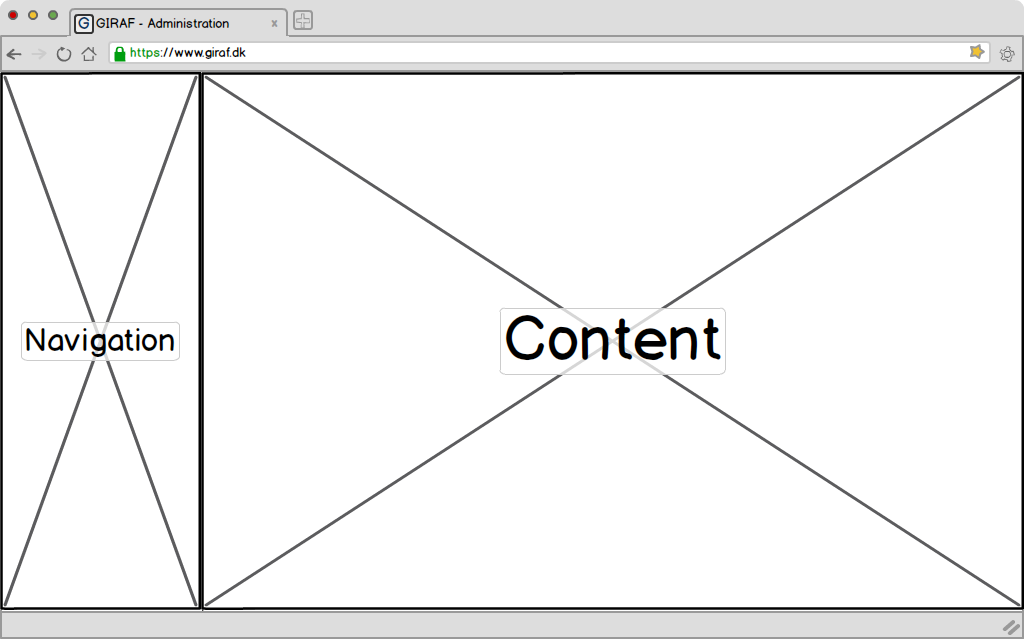
\includegraphics[width=1\textwidth]{images/mockup/displayMode.png}
\caption{General idea of building web-pages.}
\label{fig:ideaWep}
\end{figure}


\section{Designing individual pages}
\subsection{Login}
The Login page is designed to be as minimal as possible. There should be no cluttered information and with a single exeption no other option than to login, the exeption being changing language. The mockup is viewable on figure \ref{fig:loginDesign}.
\begin{figure}[p]
\centering
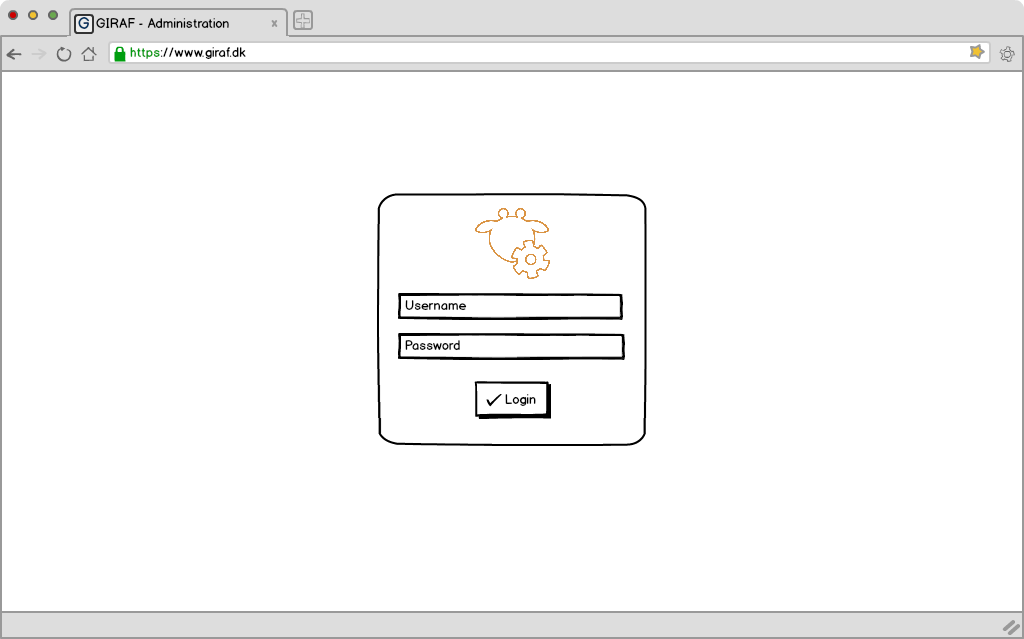
\includegraphics[width=1\textwidth]{images/mockup/login.png}
\caption{Login}
\label{fig:loginDesign}
\end{figure}

\subsection{Navigation}
Navigation was one the design items that went through a lot of small changes. The general idea being that it should look an feel natural to an android user. This being that the navigation bar conforms to a principle about accessability so that there is no foldout points or other elements that would be considered diffucult to get to on a touch screen. On the mockups each menu category has a little image next to it, this is changed so that now the first letter is capatalised and uses a bigger font than the rest of the test. If a user with administrator rights login he will be able to see all menu items but if a user with degrated rights logs in he will only see Own Profile, Pics Manager and App Manager further information about  department for an example is then accesible through own profile without editting rihgts.  A mockup showing the navigation and the profile page is figure \ref{fig:own_profileDesign}.
\begin{figure}[p]
\centering
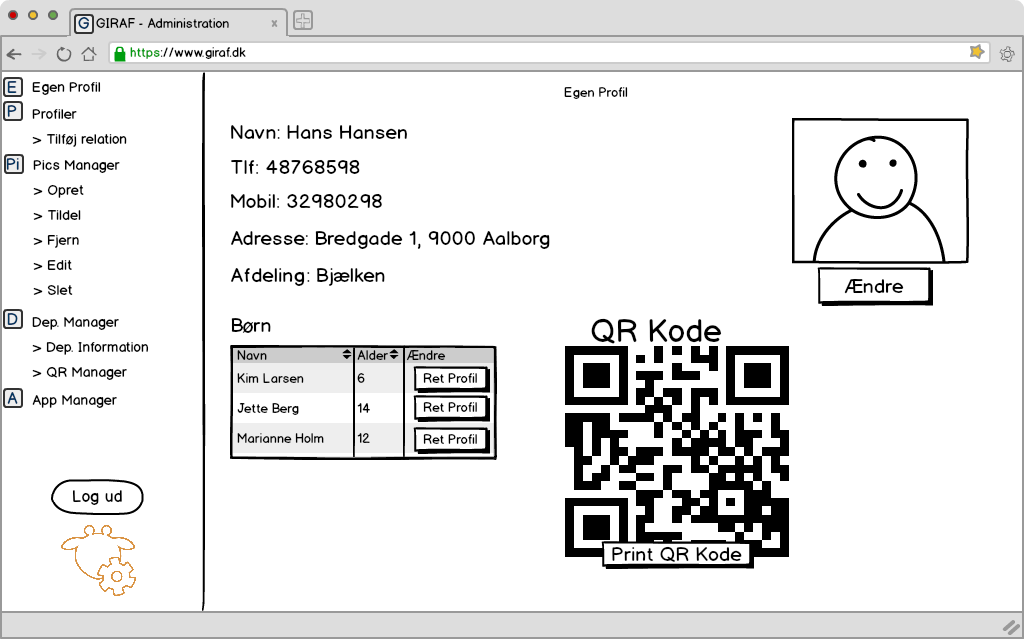
\includegraphics[width=1\textwidth]{images/mockup/egenProfil.png}
\caption{Navigation and Profile page}
\label{fig:own_profileDesign}
\end{figure}

\subsection{Profile Page}
The profile page is the page that is showed when a user logs in. It should have information about the user as well as information about linked profiles such as attached children, parents or pedagouges. A user should also be able to edit his own information as well as attached childrens information. As a result of our usability test \ref{chap:usabilityTesting} the current design used does not include the abillity to change ones QR-code. Instead only the Ddepartment manager has that abillity. A mockup showing the navigation and the profile page before usability testing is figure \ref{fig:own_profileDesign}.

\subsection{Profiles}
It is based on the idea that having a complete overview of how things are linked sometimes gives a better overview and therefore it is designed such that all links between pedagouges, children and their parents are displayed in an easy to comprehend way. To do this we agreed upon a single table approach which gracefully full-fills the comprehension wanted. This is even more underpinned when color coding is applied to guide the user.
\subsubsection*{Create Profile}
The title basecally says everything. Here the point is that one, if privileged, would be able to create other profiles. A number of input fields as weel as the option to select which type of user one want to create is what this page consits of.
\subsubsection*{Add relation}
Here a privileged user should be able to create relations or links between other profiles. A scenario would be that a child profile has just been created and it should now be linked to it's alreade created parents. This procedure should take place here.

\subsection{Pics Manager}
Pics Manager is based opun having the capabillity to create, add, remove, edit and delete pictograms which all are designed to the same principles of easy accessibility as the rest of the system. Pics Manager should not be accessible on tablets. This is mostly due to the fact that sepperate applications has been developed for it's primary purpose. It should instead open theese apllications and the user should not be bothered by this. The different components design should have the same look and feel as the android application but take advantage of the fact that they are run on a dektop computer and not a tablet.
\subsubsection*{Create}
Originalle named Make this tool should supply the user with the capability to create pictograms in the database.
\subsubsection*{Add}
Add pictograms to users.
\subsubsection*{Remove}
Remove pictograms from users.
\subsubsection*{Edit}
Enables the user to edit pictograms that the user has available.
\subsubsection*{Delete}
If a user own a pictogram he can delete it permanently from the database.

\subsection{Department Manager}
Enables a privileged user to edit department infomartion and view a shortlist of attached pedagouges.
\subsubsection*{Department Information}
Essentially the same as Department Manager but displays the information as an unprivileged user would see it. An unprivileged user accesees the page through a link on his profile page.
\subsubsection*{QR mamanger}
Enables a privileged user to change users qr-codes. This is also one of the pages that have gone through a number of deisgn itterations. as viewable in \ref{apx:mockups} it originally had three sub items but was refinded to a single page with a much more comprehensive layout. This enables the user to complete a given task much more easaly. A screenshot of the current lauoyt is \ref{fig:qrManagerCurrentDesign}
\begin{figure}[p]
\centering
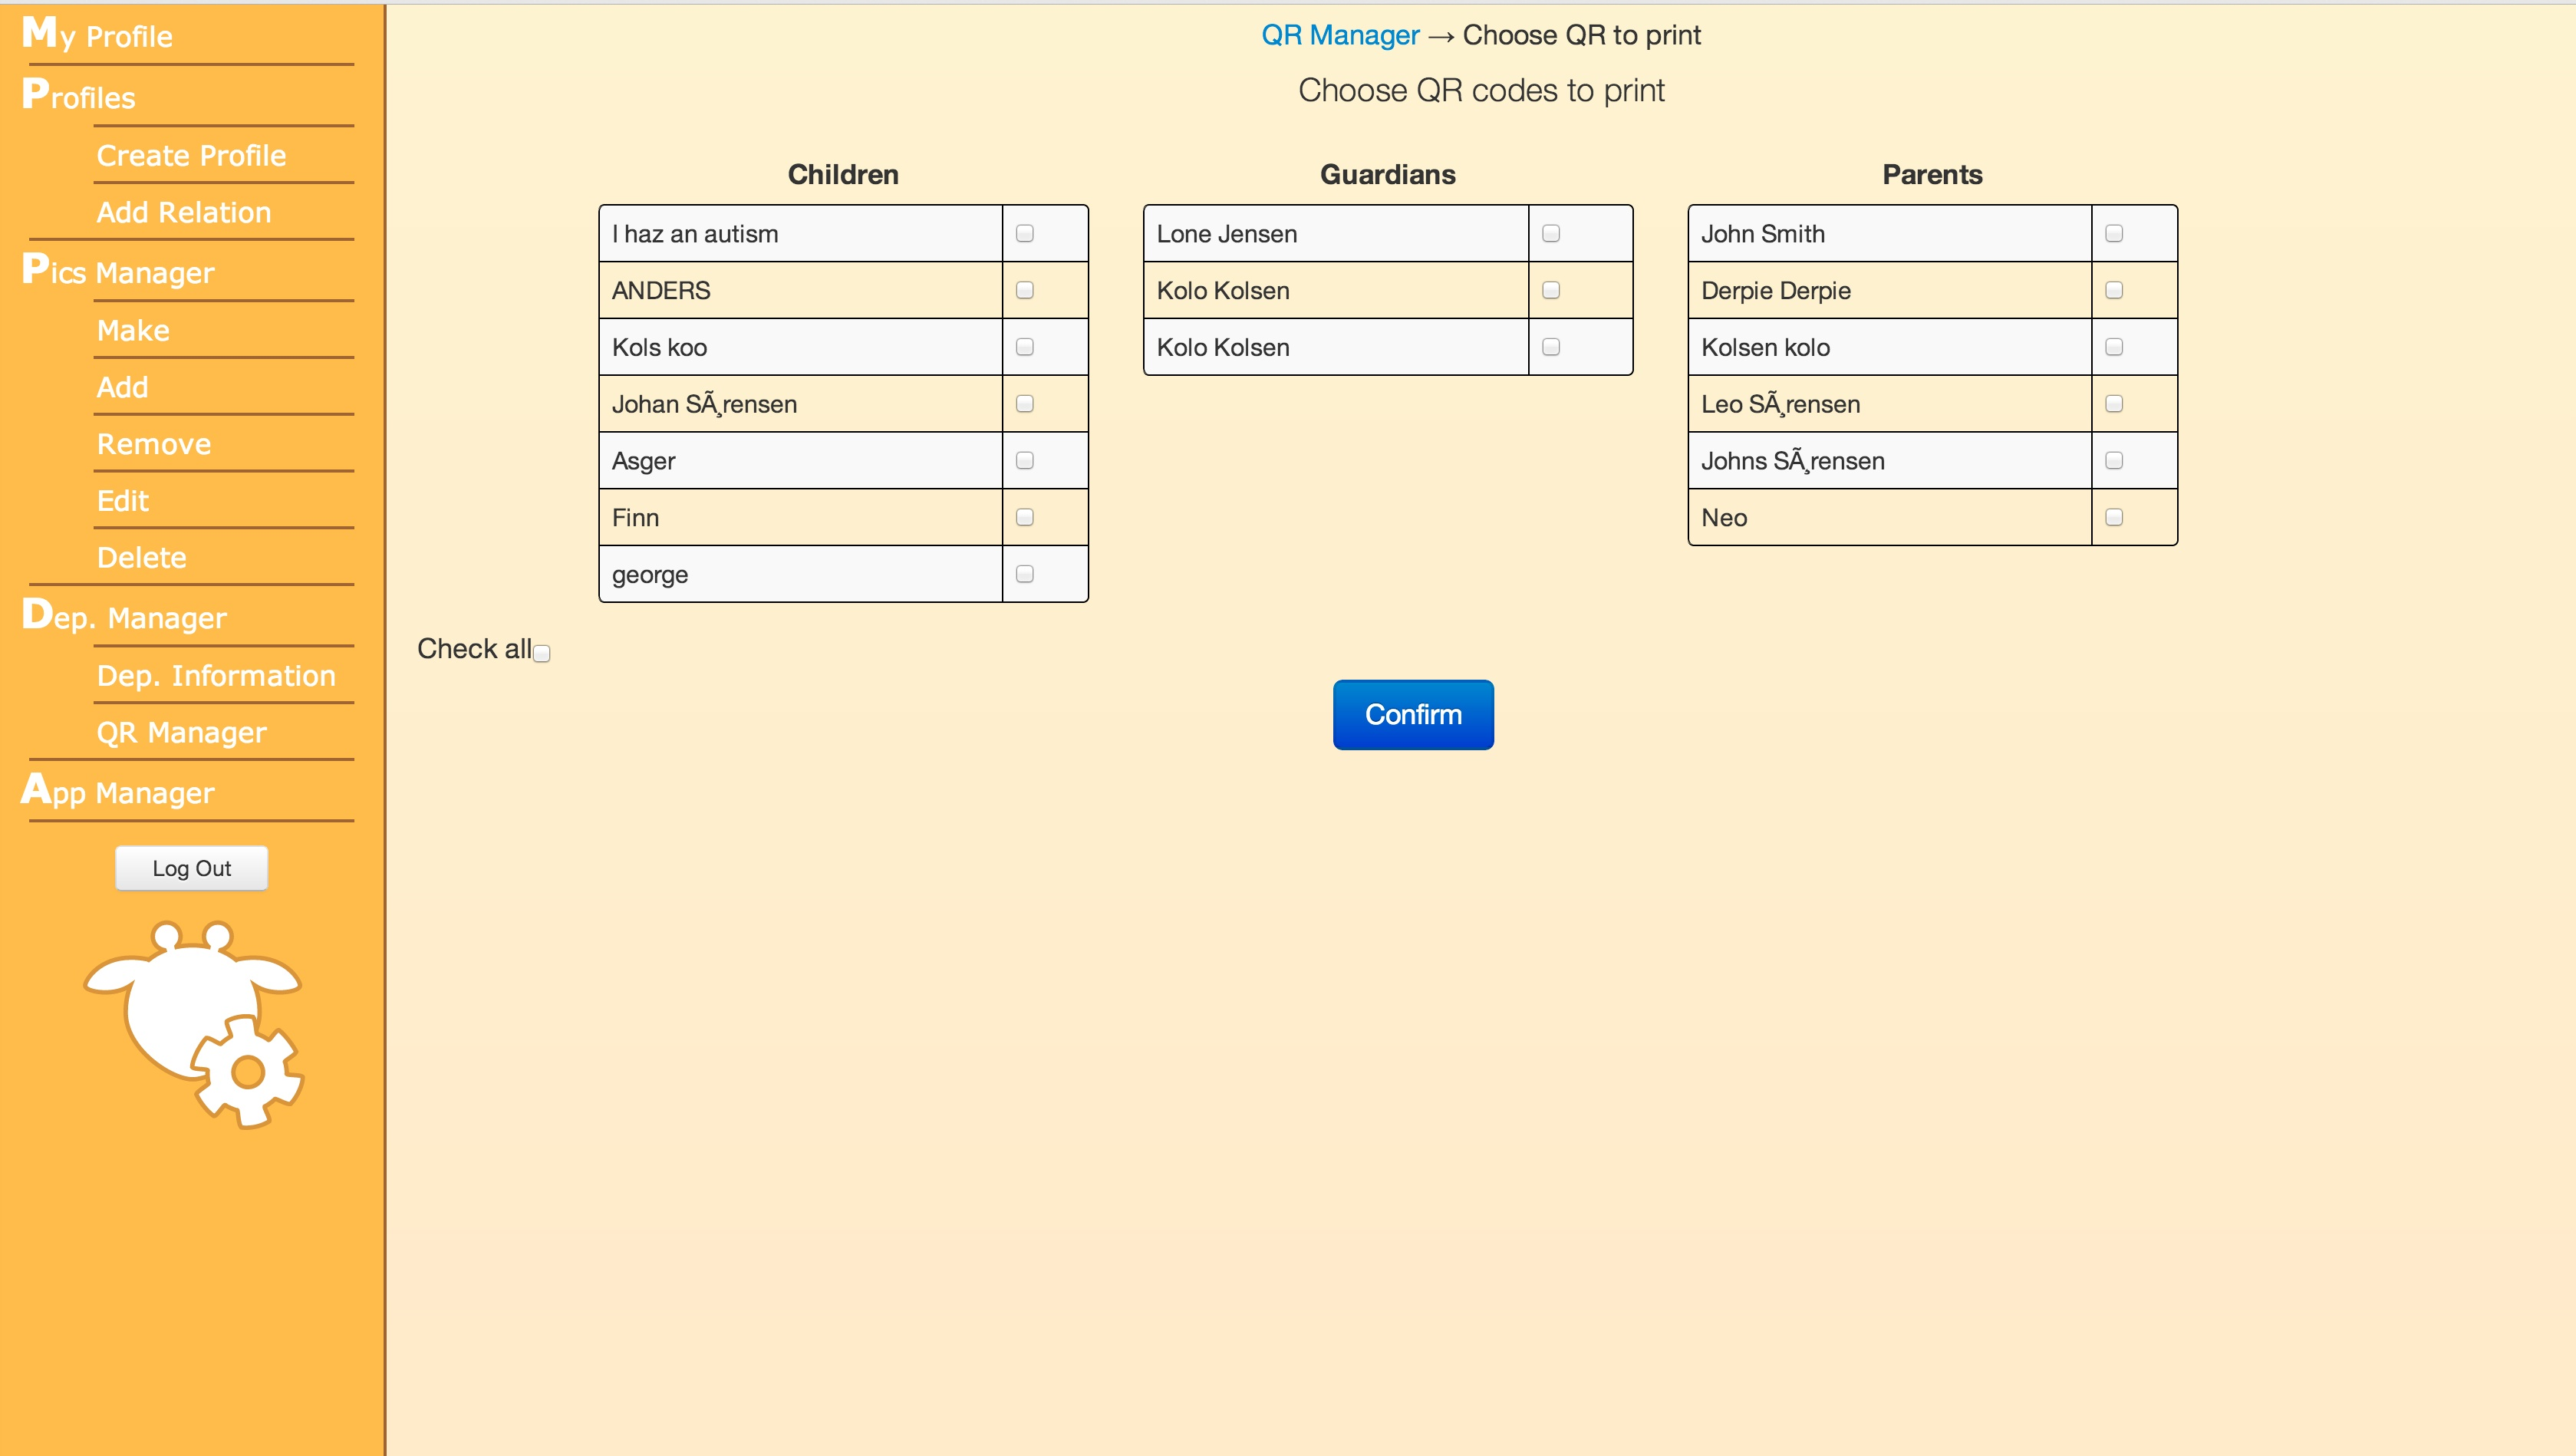
\includegraphics[width=1\textwidth]{images/mockup/qrManagerCurrent.jpg}
\caption{Current design of QR manager}
\label{fig:qrManagerCurrentDesign}
\end{figure}